\documentclass[11pt,a4paper,twoside,graphicx,color]{article}
%
\usepackage[margin=2cm]{geometry}
\usepackage[margin=2cm]{geometry}
\usepackage[pdftex]{graphicx}
\usepackage{color}
\usepackage{txfonts}
\usepackage{paralist}
\usepackage[numbers]{natbib}
\setlength{\bibsep}{0.0pt}
\usepackage{amssymb}
\usepackage[breaklinks, colorlinks, citecolor=blue, linkcolor=MyBlue, urlcolor=RoyalPurple, colorlinks=true, linkcolor=blue, debug, baseurl=' ']{hyperref}
%
\textheight 260mm
\textwidth 178mm
\oddsidemargin -8mm
\evensidemargin -8mm
\marginparwidth 50pt
\topmargin -22mm
\brokenpenalty=10000
\sloppy
%
\bibpunct{(}{)}{;}{a}{}{,} 
\bibliographystyle{aa}
%-------------------------------------------------------------------
\begin{document}
\section{Abstract}
We propose to observe two of the Planck tSZ discovered clusters of galaxies as a pilot project to test the feasibility of lensing studies with the GTC.
The clusters proposed here, PSZ1 G045.85+57.71 and PSZ1 G046.13+30.75, have been recently observed in SZ (at 150 and 260 GHz) with the NIKA camera, at the IRAM 30~m telescope. NIKA complements Planck observations with an high angular resolution follow-up (~20 arc sec at 150~GHz). The same clusters are also part of an XMM program, and we then also dispose of high-quality X-ray data for them. The tSZ and X-ray signals probe the diffuse baryonic gas component of galaxy clusters. Under the hypothesis of hydrostatic equilibrium, we can use these baryonic tracer to recover the cluster total mass. Through gravitational lensing we can instead directly explore the distribution of the dark matter component, which largely dominates the cluster total mass. The goal of this proposal is then to test the GTC lensing capabilities, and the complementarity with NIKA observations, in view of the NIKA2 large program aiming at observing 50 objects, to explore the properties of the cluster population beyond the local Universe (z $>$ 0.5). The complementarity of the tSZ and gravitational lensing can in fact allow studying how does the distribution both dark matter and gas evolve with redshift and the complex interplay between the gravitational and non-gravitational processes governing the cluster astrophysics.

\section{Scientific justification}
%open questions in cosmology with clusters

%---------- Clusters are good for cosmology
Clusters of galaxies provide valuable information concerning the evolution and composition of the Universe, and the formation of large scale structures. The observable properties of clusters reflect their formation through hierarchical gravitational collapse, by accretion and merging of smaller sub-clusters and groups, as well as the contribution of non-gravitational processes (e.g. AGN feedback and supernova-driven galactic winds) that can affect their observed properties to a large extent \citep[e.g.][]{sembolini2014}. Consequently, a detailed characterization of the both the dark matter (mainly governed by gravity) and baryonic  (governed by both gravity and radiative processes) components is a mandatory step to achieve a better control on the astrophysical systematics that represent the limit of cluster derived cosmological constraints. In order to use any cluster catalog to put constraints on the Universe content and evolution, we need an observable to mass relation. And at present we are limited by systematic uncertainties in the mass normalization of the baryonic mass proxies provided by X-ray and SZ, as recently shown by \cite{planck_nc_2015}. 

By using the high angular resolution of the NIKA (and the future NIKA2) camera we can explore the details of the pressure distribution within clusters, which means the details of the distribution of the ICM thermal energy. This will for example allows us to study the impact of shocks due to merging events on the tSZ global properties (i.e. the integrated SZ signals, $Y$), that is used as a mass proxy for cosmological purposes. But SZ and X-ray mass estimates are based on a strong assumption about how the dark matter and ICM baryonic component are related. This is the hydrostatic equilibrium hypothesis, which might provide biased mass estimates, as lensing based studies have shown \citep[e.g. ][]{WtG2014}. Gravitational lensing provides in fact a completely independent measure of the cluster total mass, being directly sensitive to the whole mass of the structure, along the line of sight. While baryonic observables provide low scatter proxies, the advantage of gravitational lensing mass estimates is that of being unbiased. Therefore,  only the the unique complementarity of multi-wavelength observations from optical, X-ray, and millimeter-wavelength via the tSZ effect, can provide a clear picture of the ongoing physics and help breaking degeneracies and systematic effects associated to each probe, which in turn affects any cosmological interpretation.

%complex interplay between the gravitational and non-gravitational processes acting on clusters is mandatory for an in-depth understanding of their astrophysics, which in turn affects any cosmological interpretation. Many open questions are the subject of active research, among which: 1) how does the distribution of galaxies, dark matter and gas evolve during cluster formation, both at small and large scales? 2) how does the resulting tridimensional geometry affect the cluster observables, in opposition to the spherical symmetry widely assumed? 3) what fraction of non-thermal component arises and how does it bias observables? 4) how do physical processes evolve during cluster formation and with redshift?

%---------- The two approaches for using clusters in cosmology
%Cosmological studies with galaxy clusters requires the use of two approaches that are intrinsically connected and complementary: 1) the detailed characterization of the physics of individual clusters, in order to better constrain the relationship between their mass and their observables; and 2) the study of statistical properties of large samples via their relation to the underlying cosmology using mass--observable scaling laws and the two point clusters correlation function (or cluster clustering), which traces the matter fluctuations on cosmological scales. In both cases, the unique complementarity of multi-wavelength observations from optical, X-ray, and millimeter-wavelength via the tSZ effect, can provide a clear picture of the ongoing physics and help breaking degeneracies and systematic effects associated to each probe.

%---------- How
In addition to the galaxy distribution, valuable in itself, optical data can be used to infer strong lensing (SL) or/and weak lensing (WL) maps which are sensitive to the projected total mass of the cluster, $\Sigma \propto \int \rho \ dl$, along the line-of-sight \citep[see][for a review]{hoekstra2013}. While SL modeling allows for a precise characterization of the mass distribution in the inner parts of the cluster, WL can be used at larger radii so that high-fidelity mass mapping is achievable over the entire cluster extension, up to the virial radius. X-ray and tSZ probe the gas physics, itself strongly related to the total mass distribution. The X-ray surface brightness is proportional to the projected electronic density ($n_e$), with a small temperature ($T_e$) dependance, as $S_X \propto \int n_e^2 \sqrt{T_e} dl$. The X-ray spectral analysis also provides temperature estimates but rapidly becomes expensive with increasing redshift, due to the large photon count required. The tSZ surface brightness is related to the integrated pressure along the line-of-sight as $\Delta I \propto f(\nu) \int n_e T_e dl$ with a characteristic spectral dependance $f(\nu)$. Conversely to X-ray, it does not suffer from cosmological dimming and it is only limited by the resolution and sensitivity of the observations. These observables provide an independent and complementary insight into the physics of galaxy clusters.

%While detailed studies of individual clusters are relatively common in the nearby Universe, it is not the case at higher redshift. Unfortunately, it is precisely at high-redshift that structure formation is the most efficient and clusters most sensitive to cosmology. Additionally, scaling relations used for cosmology, which link observables to the cluster mass, are calibrated using nearby clusters and standard evolution. Checking their evolution with redshift is therefore mandatory for using valuable high-redshift clusters in cosmological cluster samples. 

%We propose is to characterize the multi-wavelength cluster properties. As a starting point, we will take advantage of a privileged access to 150 and 260 GHz high resolution ($<20$ arcsec) tSZ NIKA (and then forthcoming NIKA2 clusters, about 50 objects at $0.5<z<1.5$, starting in early 2016) data of intermediate and high-redshift clusters. At these redshifts ($z \gtrsim 0.5$) the Planck tSZ maps are unresolved but will be used to constrain the overall tSZ flux of each system. We will use available X-ray data, such as the ones obtained by XMM (which are already planed to be combined systematically to that of NIKA2), for constraining the electronic density of the selected clusters. HST optical images and SL surface mass models are already available for most of the NIKA clusters \citep[e.g.][]{zitrin2011,postman2012}. The NIKA2/XMM clusters will also be combined with overlapping optical data obtained with available optical surveys to cross correlate the WL mass and galaxy distribution. 

In the future, with the NIKA2 cluster sample (50 objects at z~$>$~0.5), this kind of study will finally permit: {\bf 1)} To test the hydrostatic equilibrium assumption (i.e. the hydrostatic mass bias) against redshift and as a function of cluster centric distance. This can be done combining resolved mass profiles from lensing (independent of the gas physics) and SZ+X-ray which assumes hydrostatic equilibrium. {\bf 2)} To quantitatively probe the amount of non-thermal support as a function of the dynamical state of the systems and along with redshift. {\bf 3)} To constrain the spatial distribution of dark matter versus the stellar content and its interplay with the baryonic mass component which will allow us to study the formation process and evolution of clusters. {\bf 4)} To constrain cluster triaxiality, as the combining of SZ, X-ray and lensing is sensitive to the line-of-sight elongation, thanks to their different sensitivities to the ICM physics. While numerical simulations suggest that clusters are triaxial, they are generally assumed to be spherically-symmetric due to the difficulty to probe the three-dimensional shape. This can lead to biases and scatters in cosmological constraints. See e.g. \cite{limousin2013} and the results by \cite{morandi2012} on a nearby cluster. 


{\bf ADD DISCUSSION ON THE 2 CLUSTERS PROPOSED: X-ray morphology vs SZ, PSZ1 G046 in SZ is less spherical than in X, but seems to better trace the galaxy distribution.}

%-------------------------------------------------------------------
\begin{table}
\begin{center}
\resizebox{\textwidth}{!} {
\begin{tabular}{|p{3.4cm}|p{1.6cm}|p{1.6cm}|p{0.6cm}|p{1.8cm}|p{7.3cm}|}
\hline
Cluster & R.A. & Dec. & $z$ & $Y_{500}$ (arcmin$^2$) & Comment \\
\hline
PSZ1 G045.85+57.71 & 15:18:20.8 & $+29$:27:37 & 0.61 & $0.82 \times 10^{-3}$& Elongated but fairly relaxed in \mbox{X-ray}. Observed with Subaru. tSZ peak at about 5 mJy/beam.\\
PSZ1 G046.13+30.75 & 17:17:05.8 & $+24$:04:25 & 0.57 & $0.77 \times 10^{-3}$ & Compact in X-rays. Observed with Subaru. tSZ peak at about 4 mJy/beam. \\
\hline
\end{tabular}
}
\end{center}
\caption{\footnotesize Brief characteristics of the proposed clusters. }
%\textcolor{red}{MACSJ0717 fait un peu tache ici. En plus si jamais on a effectivement besoin de le re-observer pour l'avoir bien a 1mm, il va falloir plutot 20 heures d'hiver que quelques heure d'ete. Donc je propose de le virer. Sinon je vous laisse justifier qu'on le met aussi.}}
\label{tab:list_gc}
\end{table}

%============================== Suporting material
\section{Supporting material}
\begin{figure}[h!]
	\centering
	\textbf{PSZ1 G045.85+57.71}\par\medskip
	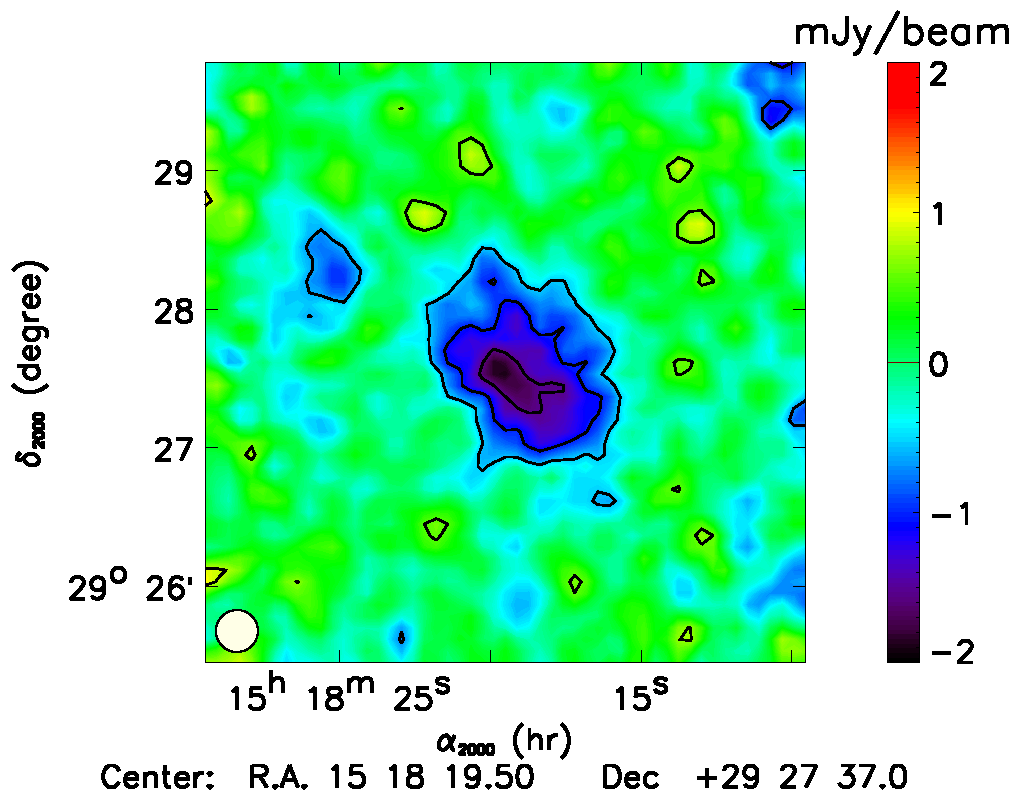
\includegraphics[width=0.4\textwidth]{PSZ1G045_map_NIKA_2mm.pdf}
	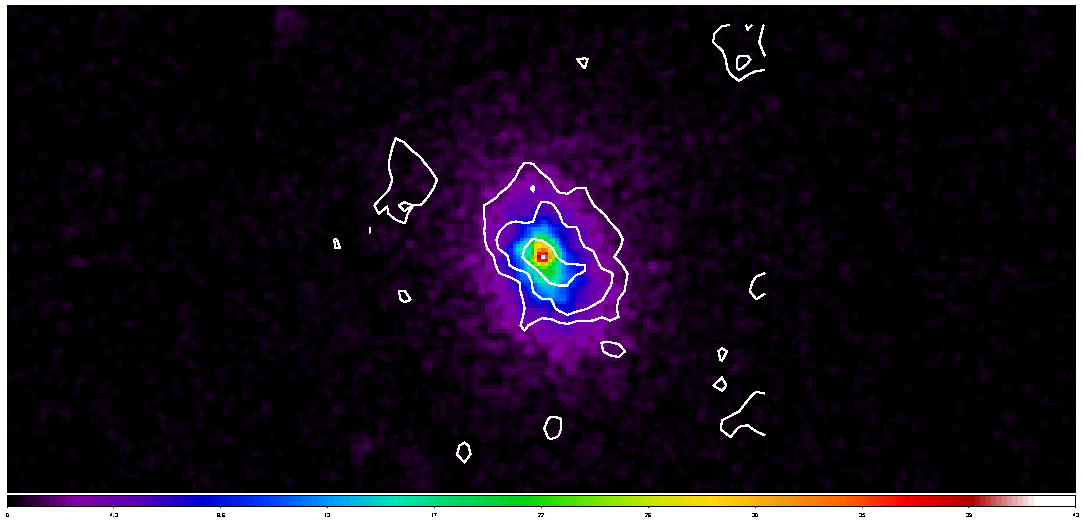
\includegraphics[width=0.5\textwidth]{PSZ1G045_X_SZcont.pdf}
	\caption{Left: NIKA tSZ map, at 150~GHz. Right: The NIKA tSZ contours (in white) are over-plotted on the X-ray photon counts map, obtained with XMM for the same cluster.}
	\label{fig:maps}
\end{figure}

\begin{figure}[h!]
	\centering
	\textbf{PSZ1 G046.13+30.75}\par\medskip
	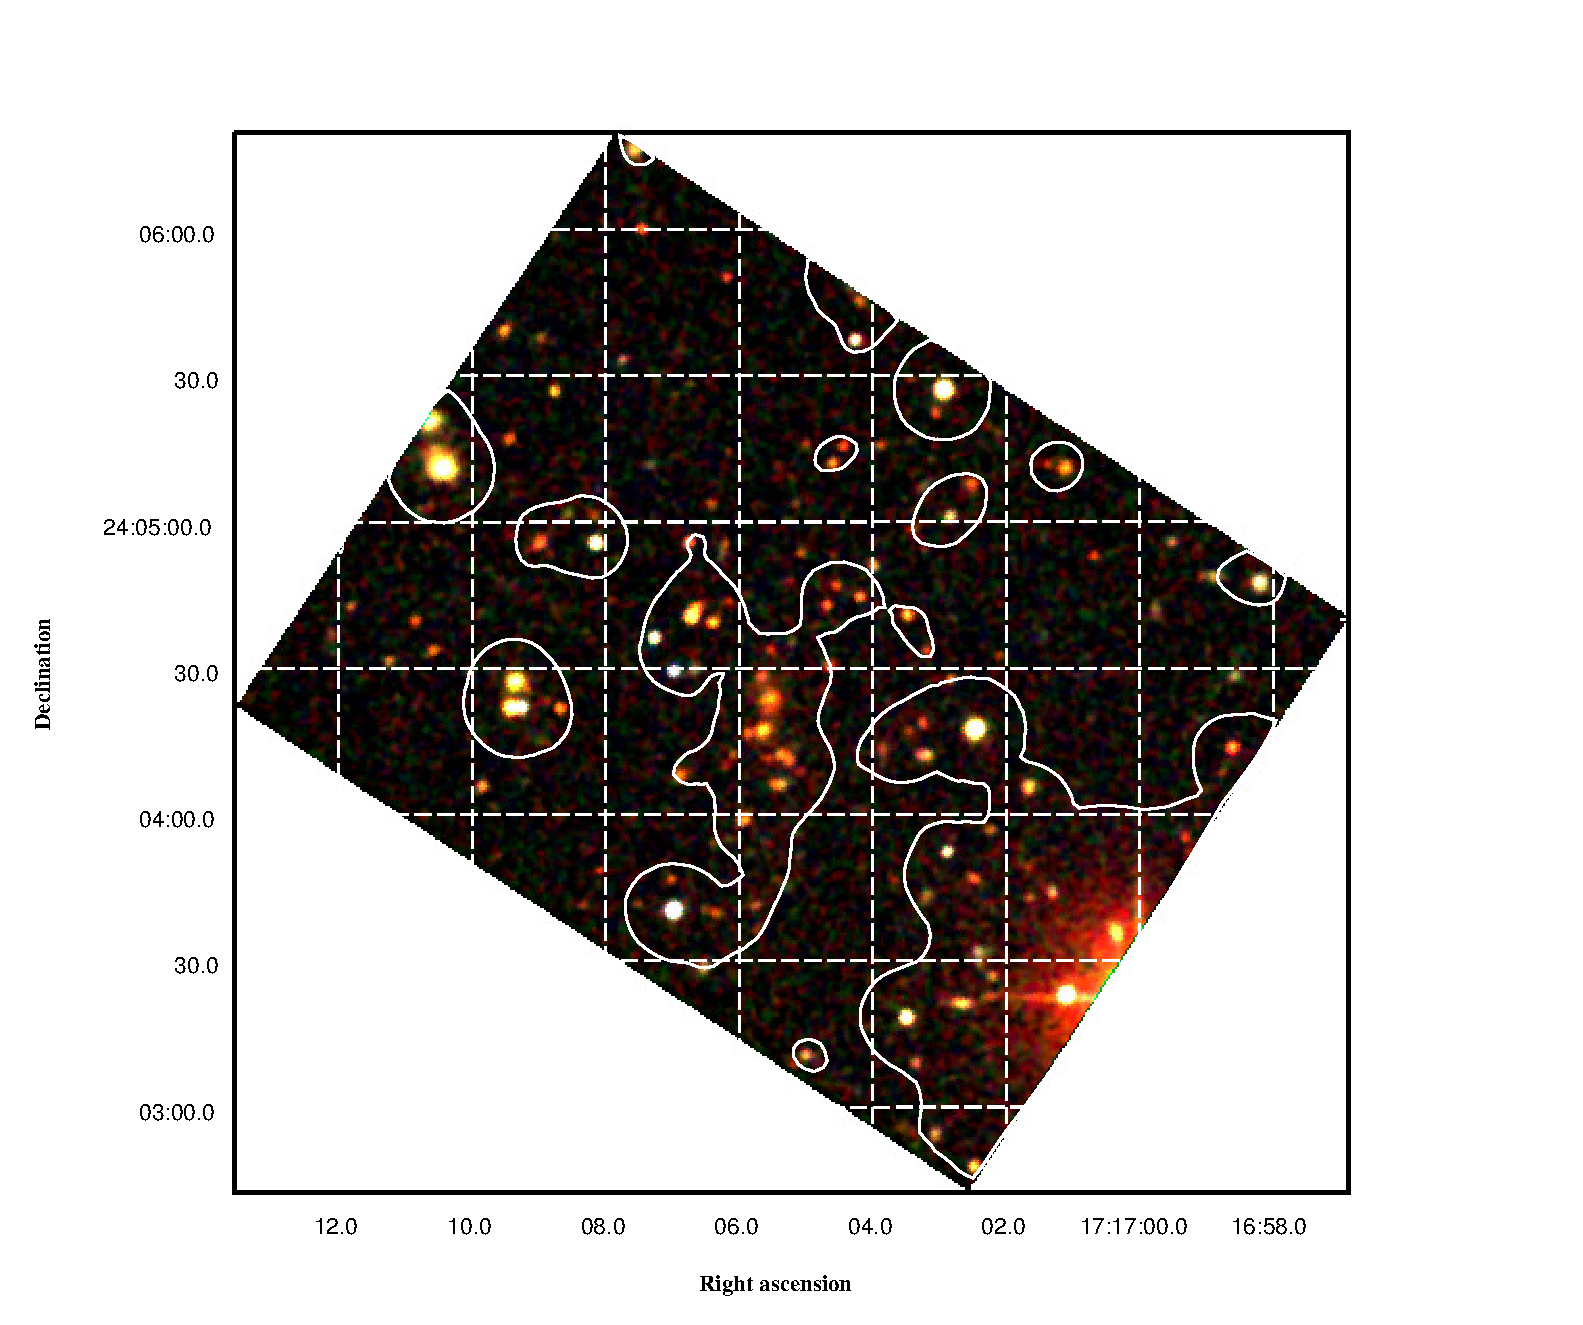
\includegraphics[trim=0.5cm 0cm 4cm 0cm, clip=true, height=6.5cm]{PSZ1G046_SDSS.pdf}
	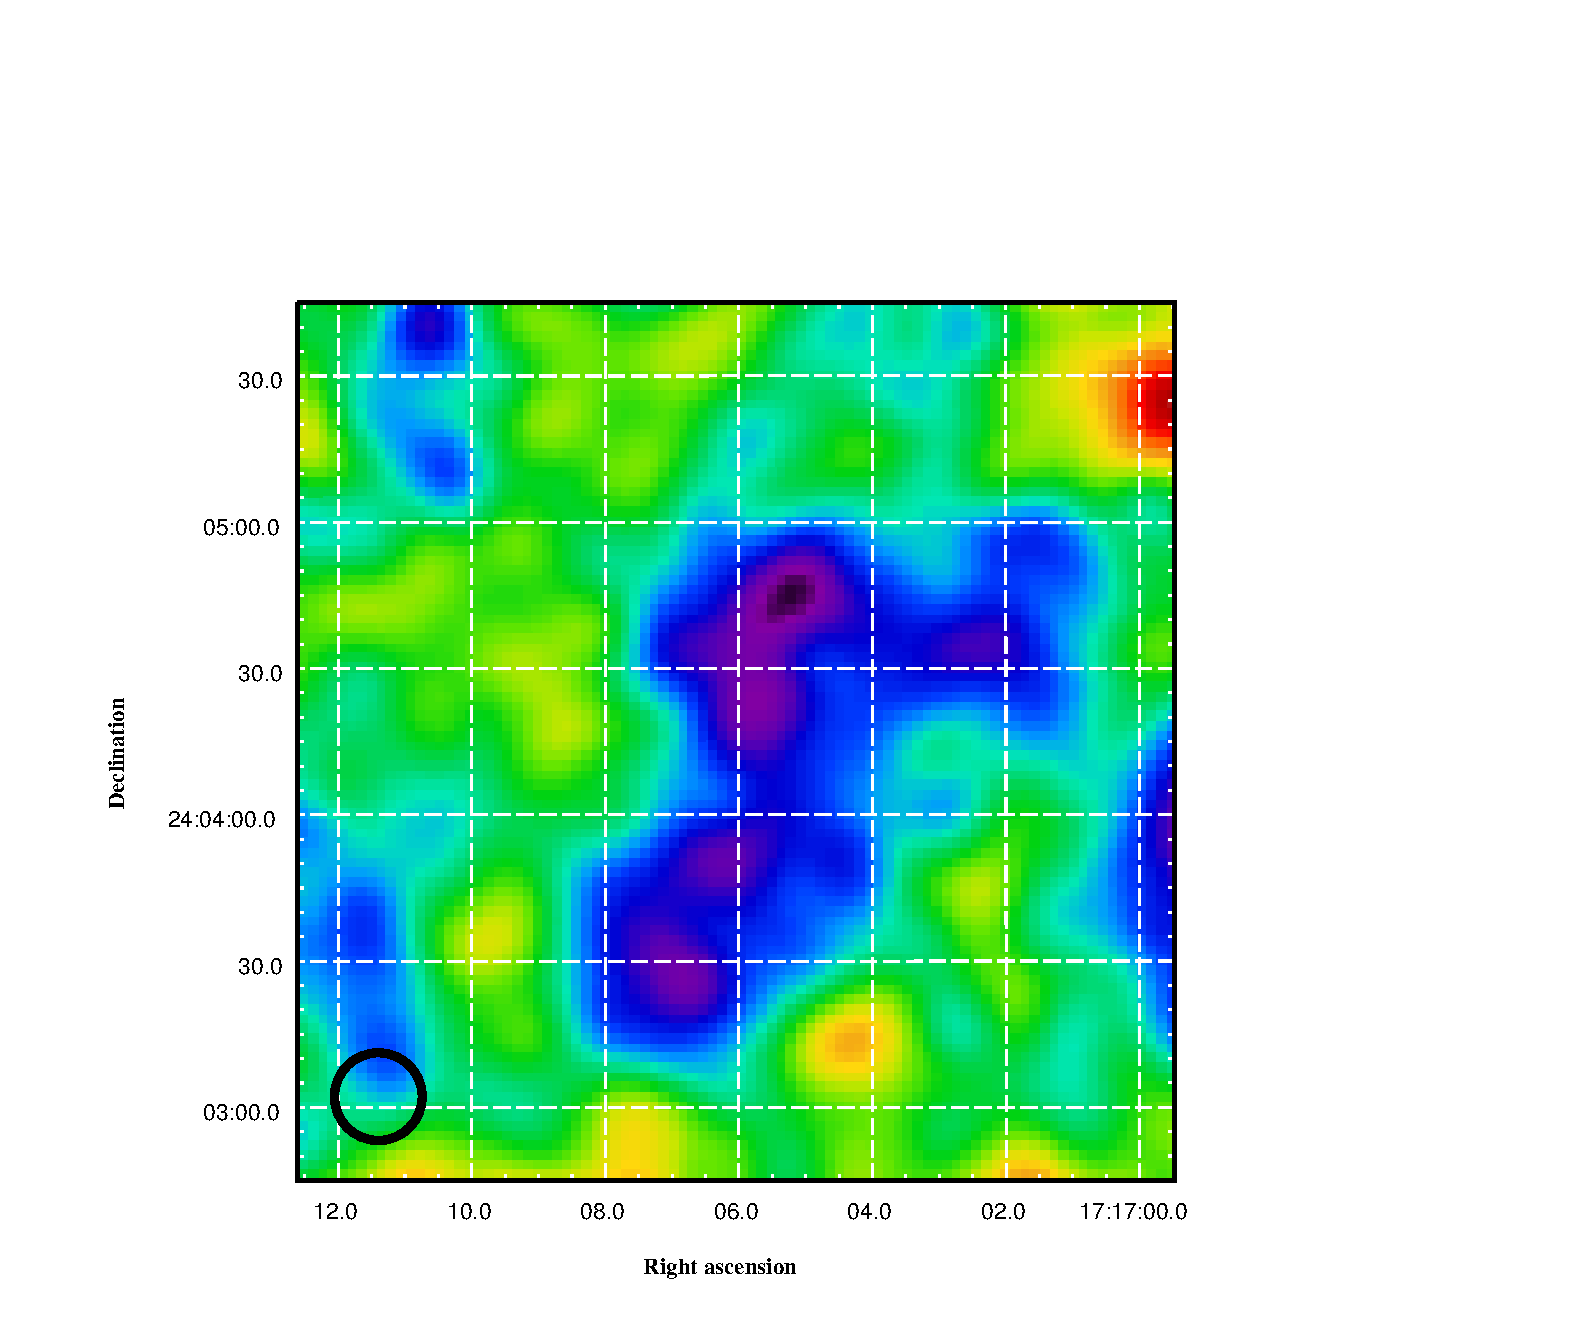
\includegraphics[trim=2.5cm 0cm 7cm 0cm, clip=true,height=6.5cm]{PSZ1G046_NIKA.pdf}
	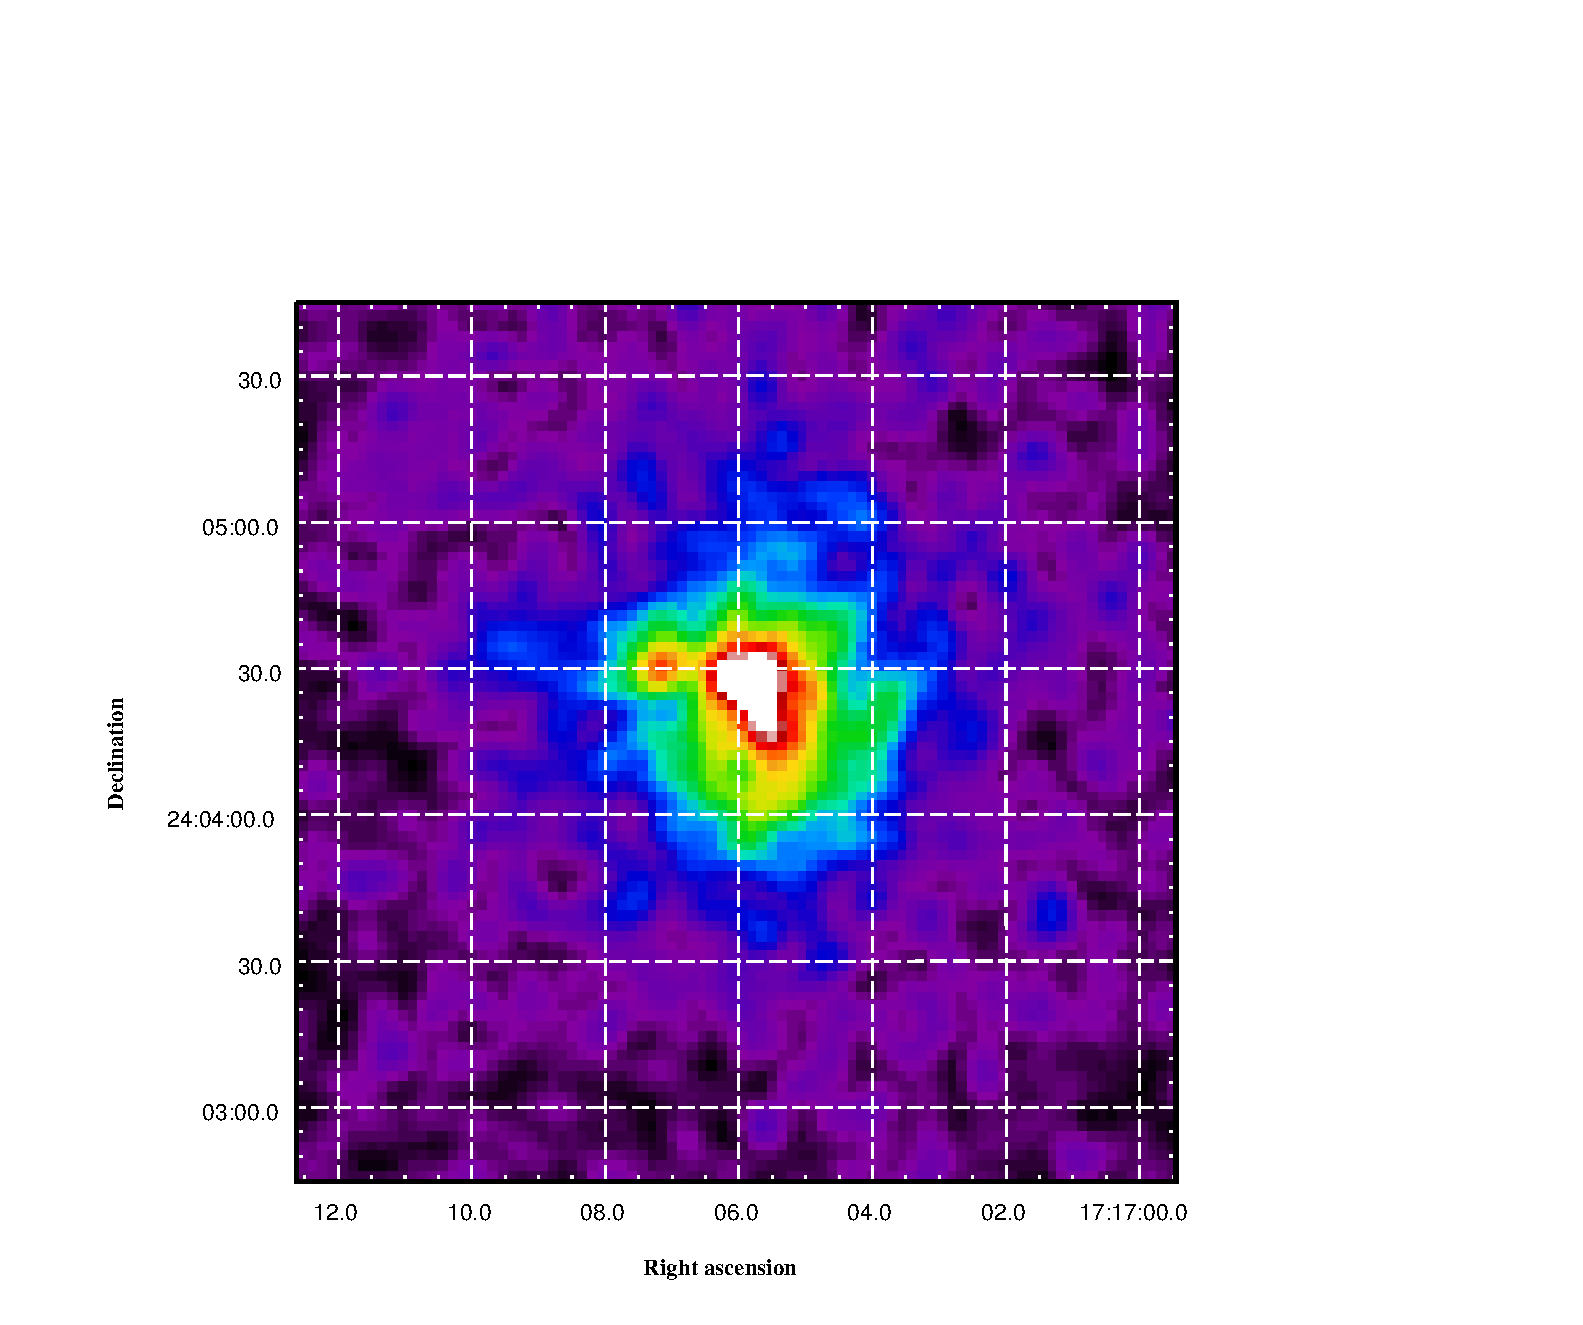
\includegraphics[trim=2.5cm 0cm 7cm 0cm, clip=true,height=6.5cm]{PSZ1G046_XMM.pdf}
	\caption{Left: SDSS i, r, and g bands composite image towards PSZ1~G046.13+30.75. The white contours provides a 5 arcsec smoothed brightness distribution in the red band, which gives an indication of the cluster galaxy distribution. Middle: NIKA tSZ map. All the data indicate an elongated morphology. Right: XMM X-ray photon count.}
	\label{fig:maps} 
\end{figure}

%%%%%%%%%%%%
\begin{thebibliography}{9}

\bibitem[Adam et al.(2013)]{adam2013}
R. Adam, B. Comis, J.-F. Mac\'ias-P\'erez, {\it et al.} (2013), A\&A in press, arXiv:1310.6237
 
 \bibitem[Adam et al.(2014b)]{adam2014b}%Moriond
R. Adam, {\it et al.} (2014b), Moriond conference, arXiv:1409.1137

\bibitem[Birkinshaw(1999)]{birkinshaw1999}
M. Birkinshaw (1999), Phys. Rep., 310, 97

\bibitem[Hoekstra et al.(2013)]{hoekstra2013}%Review lensing
H. Hoekstra, M. Bartelmann, H. Dahle {\it et al.} (2013), SSR, 177, 75-118, arXiv:1303.3274

\bibitem[Limousin et al.(2012)]{limousin2012}%MACSJ0717 lensing
M. Limousin, H. Ebeling, J. Richard {\it et al.} (2012), A\&A, 544, A71, arXiv:1109.3301

\bibitem[Limousin et al.(2013)]{limousin2013}%Review triaxial
M. Limousin, A. Morandi, M. Sereno {\it et al.} (2013), SSR, 177, 155-194, arXiv:1210.3067

\bibitem[Morandi et al.(2012)]{morandi2012}%SZ/X/lensing analysis of Abell 1835
A. Morandi, M. Limousin, J. Sayers, {\it et al.} (2012), MNRAS, 425, 2069-2082, arXiv:1111.6189

\bibitem[Mroczkowski et al.(2012)]{mroczkowski2012}
T. Mroczkowski, S. Dicker, J. Sayers {\it et al.} (2012), ApJ, 761, 47, arXiv:1205.0052

\bibitem[Planck Collaboration (2015)]{planck_nc_2015}%Planck
Planck Collaboration  (2015), arXiv:1502.01597

\bibitem[Postman et al.(2012)]{postman2012}%CLASH
M. Postman, {\it et al.} (2012), APJS, 199, 25, arXiv:1106.3328

\bibitem[Sembolini et al.(2014)]{sembolini2014}%Baryons in simu
F. Sembolini, M. De Petris, G. Yepes, {\it et al.} (2014), MNRAS, 440, 3520-3531, arXiv:1309.5387

von der Linden
\bibitem[von der Linden et al.(2014)]{WtG2014}%WtG
A. von der Linden, {\it et al.} (2014), MNRAS, 439, 2-27, arXiv:1208.0597
	
\bibitem[Zitrin et al.(2009)]{zitrin2009}
A. Zitrin, T. Broadhurst, Y. Rephaeli, S. Sadeh, {\it et al.} (2009), ApJ, 707, 102

\bibitem[Zitrin et al.(2011)]{zitrin2011}%SL model MACSJ0717
A. Zitrin (2011), MNRAS, 410, 1939-1956, arXiv:1002.0521

\end{thebibliography}

\end{document}
